% ==============================================================
% CAPÍTULO 5 — ANÁLISE ORGANIZACIONAL
% ==============================================================

\chapter{Análise Organizacional}
\label{cap:analise-organizacional}

Esta seção analisa a estrutura organizacional da Capim Software a partir de quatro perspectivas complementares: hierarquia interna, Estrela de Galbraith, configuração de Mintzberg e análise SWOT. As informações têm como base a entrevista com Lucas Mathias, PM de experimentos e integrante do time fundador \cite{capimentrevista2026}, e dados secundários.

\section{Hierarquia e Ritos de Coordenação}

A Capim, com cerca de 150 colaboradores em 2026, organiza-se em squads multidisciplinares por produto, com coordenação central exercida pela Diretoria de Produto. Cada squad é autônomo na operação, mas alinhado estrategicamente por meio de dois ritos formais, sintetizados na Figura~\ref{fig:organograma} e detalhados na Tabela~\ref{tab:ritos} (Capítulo~\ref{cap:processo-decisorio}).

\begin{figure}[h]
  \caption{Organograma resumido da Capim Software}
  \label{fig:organograma}
  \centering
  \resizebox{\textwidth}{!}{%
  \begin{tikzpicture}[
      node distance=10mm and 6mm,
      box/.style={draw, rounded corners, align=center, minimum width=32mm, minimum height=9mm, font=\small},
      every edge/.style={draw, -{Stealth[length=2mm]}}
    ]
    \node[box, fill=gray!15] (ceo) {CEO};
    \node[box, below=of ceo] (dp) {Diretoria de Produto};
    \node[box, right=18mm of dp] (tech) {Liderança de Tecnologia};

    \node[box, below=14mm of dp, xshift=-57mm] (saas) {Squad\\SaaS};
    \node[box, below=14mm of dp, xshift=-19mm] (bnpl) {Squad\\BNPL/POS};
    \node[box, below=14mm of dp, xshift=19mm] (sust) {Squad\\Sustentação};
    \node[box, below=14mm of dp, xshift=57mm] (exp) {Squad\\Experimentos};

    \draw (ceo) edge (dp);
    \draw (ceo) edge (tech);
    \draw (dp) edge (saas);
    \draw (dp) edge (bnpl);
    \draw (dp) edge (sust);
    \draw (dp) edge (exp);

    \node[draw, dashed, rounded corners, fit=(ceo)(dp)(tech), inner sep=4mm, label={[font=\scriptsize]above right:Comitê Estratégico (semanal)}] {};
  \end{tikzpicture}}
  \legend{Fonte: elaborado pelos autores. Os squads de Sustentação e Experimentos e os ritos de coordenação são confirmados pela entrevista; a separação SaaS/BNPL-POS é uma reconstrução dos autores a partir das linhas de produto descritas, não um organograma oficial da empresa.}
\end{figure}

\section{Estrela de Galbraith}
\label{sec:galbraith}

O modelo de Galbraith avalia o alinhamento entre cinco dimensões organizacionais, classicamente representadas como uma estrela de cinco pontas (Figura~\ref{fig:galbraith-estrela}). A análise para a Capim em cada uma delas é detalhada a seguir.

\begin{figure}[h]
  \caption{As cinco dimensões da Estrela de Galbraith}
  \label{fig:galbraith-estrela}
  \centering
  \begin{tikzpicture}[font=\small]
    \node[regular polygon, regular polygon sides=5, draw, minimum size=4.5cm,
          fill=gray!8, rounded corners=1pt] (p) {};
    \foreach \ang/\name in {90/Estratégia, 162/Estrutura, 234/Processos,
                            306/Recompensas, 18/Pessoas} {
      \node[draw, rounded corners, fill=gray!15, font=\footnotesize]
            at (\ang:3.0cm) {\name};
      \draw[-{Stealth[length=2mm]}, gray!60] (p.center) -- (\ang:2.0cm);
    }
    \node[font=\scriptsize\itshape, gray!70] at (p.center) {alinhamento};
  \end{tikzpicture}
  \legend{Fonte: elaborado pelos autores a partir do modelo de Galbraith.}
\end{figure}

\begin{description}
  \item[Estratégia] Aprofundar penetração em odontologia via ecossistema integrado (crédito + gestão + maquininha + carnê). Foco em ``agenda cheia e rentável'' para clínicas. Crescimento por dois caminhos: melhorias incrementais nos produtos existentes e \textit{home runs} experimentais (como o modelo B2C).
  \item[Estrutura] Squads autônomos por produto, com coordenação central da Diretoria de Produto. Organização enxuta (\textasciitilde150 pessoas) e horizontal nas decisões operacionais.
  \item[Processos] Combinação adaptada de Scrum (\textit{sprints}, \textit{boards}) com \textit{stage-gates} internos: Garagem~2 $\rightarrow$ Garagem~1 $\rightarrow$ Rua. Progressão controlada pelo número de clínicas expostas (5--10 $\rightarrow$ 50--100 $\rightarrow$ 500+). Métrica de sucesso por iniciativa, revisável durante o projeto.
  \item[Recompensas] Tema não aprofundado na entrevista. Indícios apontam para reconhecimento por autonomia, \textit{ownership} e exposição direta a problemas estratégicos junto ao CEO.
  \item[Pessoas] Entrevistado e fundadores com passagem por MBA fora do Brasil, segundo relato. Cultura de iteração rápida, uso intensivo de IA (Claude, Cursor) e proximidade com o usuário final.
\end{description}

As cinco dimensões mostram-se majoritariamente alinhadas: estratégia experimental sustentada por estrutura enxuta, processos adaptáveis e pessoas culturalmente engajadas. A dimensão de processos, contudo, é examinada com maior profundidade no Capítulo~\ref{cap:processo-decisorio}, onde se mostra que o mesmo arranjo de \textit{stage-gates} adaptado é aplicado de forma relativamente uniforme a projetos de incerteza muito distinta.

\section{Configuração de Mintzberg}
\label{sec:mintzberg}

A análise indica que a Capim se enquadra majoritariamente como adhocracia operacional, configuração típica de organizações cuja atividade central é a inovação. O mecanismo de coordenação predominante é o ajuste mútuo, exercido por meio das reuniões quinzenais e semanais já descritas, em detrimento da padronização rígida de processos. A parte-chave da organização é o núcleo operacional -- os times de produto --, com forte assessoria de apoio em design, engenharia e funções de suporte. Em termos de parâmetros de design, a empresa apresenta estrutura orgânica, especialização horizontal, dispositivos de ligação entre squads e descentralização seletiva das decisões. Os fatores contextuais reforçam esse enquadramento: ambiente dinâmico, tecnologia sofisticada (software e IA) e uma organização ainda jovem, de porte médio.

Há uma exceção: o squad de sustentação apresenta traços mais burocráticos, com fluxos de trabalho mais previsíveis. Ainda assim, mesmo essa equipe se engaja em inovações incrementais, como a migração automática de sistemas legados, o que mantém a adhocracia como configuração dominante na empresa como um todo.

\section{Análise SWOT}
\label{sec:swot}

A Figura~\ref{fig:swot-quadrante} sintetiza os pontos centrais da análise no formato clássico de quadrante; a Tabela~\ref{tab:swot} detalha a lista completa.

\begin{figure}[h]
  \caption{Síntese da análise SWOT da Capim}
  \label{fig:swot-quadrante}
  \centering
  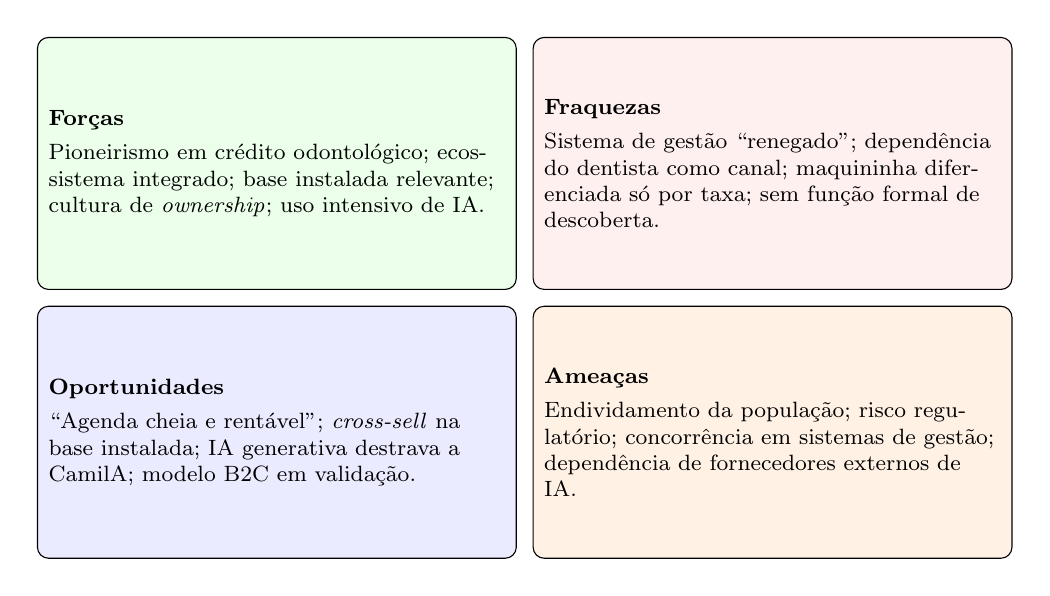
\begin{tikzpicture}[font=\footnotesize,
      cell/.style={draw, rounded corners, text width=58mm, align=left,
                   inner sep=4pt, minimum height=32mm}]
    \matrix[row sep=2mm, column sep=2mm] {
      \node[cell, fill=green!8] {\textbf{Forças}\par\smallskip
        Pioneirismo em crédito odontológico; ecossistema integrado; base instalada relevante; cultura de \textit{ownership}; uso intensivo de IA.}; &
      \node[cell, fill=red!6] {\textbf{Fraquezas}\par\smallskip
        Sistema de gestão ``renegado''; dependência do dentista como canal; maquininha diferenciada só por taxa; sem função formal de descoberta.}; \\
      \node[cell, fill=blue!8] {\textbf{Oportunidades}\par\smallskip
        ``Agenda cheia e rentável''; \textit{cross-sell} na base instalada; IA generativa destrava a CamilA; modelo B2C em validação.}; &
      \node[cell, fill=orange!10] {\textbf{Ameaças}\par\smallskip
        Endividamento da população; risco regulatório; concorrência em sistemas de gestão; dependência de fornecedores externos de IA.}; \\
    };
  \end{tikzpicture}
  \legend{Fonte: elaborado pelos autores a partir da entrevista com Lucas Mathias (2026). Versão completa na Tabela~\ref{tab:swot}.}
\end{figure}

\begin{table}[h]
  \centering
  \caption{Análise SWOT da Capim -- detalhamento}
  \label{tab:swot}
  \begin{tabularx}{\textwidth}{XX}
    \toprule
    \textbf{Forças} & \textbf{Fraquezas} \\
    \midrule
    Pioneirismo em crédito odontológico no ponto de venda &
    Sistema de gestão tratado internamente como produto ``renegado'' \\
    Ecossistema integrado (crédito, gestão, maquininha, carnê) &
    Dependência do dentista como canal de venda do crédito \\
    Base instalada: 6.000+ clínicas, R\$~450M+ em crédito originado, 70 mil+ pacientes &
    Maquininha diferenciada principalmente por taxa \\
    Cultura de \textit{ownership} e capacidade de iteração rápida &
    Portfólio concentrado em uma única vertical (odontologia) \\
    Uso intensivo de IA no produto e na operação interna &
    Iniciativas congeladas aguardando maturação tecnológica (caso CamilA) \\
    Time fundador qualificado e ainda atuante na empresa &
    Ausência de função formal de descoberta/geração de ideias (ver Capítulo~\ref{cap:processo-decisorio}) \\
    \bottomrule
  \end{tabularx}

  \vspace{2mm}
  \begin{tabularx}{\textwidth}{XX}
    \toprule
    \textbf{Oportunidades} & \textbf{Ameaças} \\
    \midrule
    Aumentar receita das clínicas via aquisição de pacientes (``agenda cheia e rentável'') &
    Endividamento da população limita a base elegível ao crédito \\
    \textit{Cross-sell} na base instalada de 6.000+ clínicas &
    Risco regulatório em crédito e meios de pagamento \\
    Avanços em IA generativa destravam iniciativas como a CamilA &
    Concorrência intensa em sistemas de gestão odontológica \\
    Expansão para verticais adjacentes (ótica, medicina geral, cirurgias eletivas) &
    Pressão sobre margens da maquininha \\
    Modelo B2C (``Uber dos dentistas'') em validação &
    Dependência de fornecedores externos de IA (Anthropic, OpenAI) \\
    Aprimoramento de modelos de risco para ampliar a aprovação responsável &
    Exposição ao macroambiente (``metáfora do elefante'' relatada pelo entrevistado) \\
    \bottomrule
  \end{tabularx}
  \legend{Fonte: elaborado pelos autores a partir da entrevista com Lucas Mathias (2026).}
\end{table}

A Capim conjuga liderança consolidada em sua categoria pioneira (crédito odontológico) com a necessidade de diversificar canais e produtos para mitigar a dependência do dentista como intermediário e a exposição ao cenário macroeconômico. Os capítulos seguintes mostram que parte dessas fraquezas e ameaças, em particular a ausência de uma função formal de descoberta de oportunidades, está diretamente relacionada a lacunas no próprio sistema de gestão da inovação da empresa.
